\documentclass{article}

% if you need to pass options to natbib, use, e.g.:
% \PassOptionsToPackage{numbers, compress}{natbib}
% before loading nips_2017
%
% to avoid loading the natbib package, add option nonatbib:
\usepackage[final, nonatbib]{nips_2017}

\usepackage[utf8]{inputenc} % allow utf-8 input
\usepackage[T1]{fontenc}    % use 8-bit T1 fonts
\usepackage{hyperref}       % hyperlinks
\usepackage{url}            % simple URL typesetting
\usepackage{booktabs}       % professional-quality tables
\usepackage{amsfonts}       % blackboard math symbols
\usepackage{nicefrac}       % compact symbols for 1/2, etc.
\usepackage{microtype}      % microtypography
\usepackage{cite}
\usepackage{graphicx}

\title{Handwriting to \LaTeX{} Markup via Neural Network}

% The \author macro works with any number of authors. There are two
% commands used to separate the names and addresses of multiple
% authors: \And and \AND.
%
% Using \And between authors leaves it to LaTeX to determine where to
% break the lines. Using \AND forces a line break at that point. So,
% if LaTeX puts 3 of 4 authors names on the first line, and the last
% on the second line, try using \AND instead of \And before the third
% author name.

\author{
  Zachary Hervieux-Moore \\
  ORF 525\\
  Final Project\\
  \texttt{zhm@princeton.edu} \\
  %% examples of more authors
  %% \And
  %% Coauthor \\
  %% Affiliation \\
  %% Address \\
  %% \texttt{email} \\
  %% \AND
  %% Coauthor \\
  %% Affiliation \\
  %% Address \\
  %% \texttt{email} \\
  %% \And
  %% Coauthor \\
  %% Affiliation \\
  %% Address \\
  %% \texttt{email} \\
  %% \And
  %% Coauthor \\
  %% Affiliation \\
  %% Address \\
  %% \texttt{email} \\
}

\begin{document}

\maketitle

\begin{abstract}
  Neural networks are well known for their image classification abilities due to
  the strong ability of convolutional neural networks (CNN) to extract features
  from an image. More recently, recurrent neural networks (RNN) are being used
  to achieve cutting edge results in language translation thanks to modern
  architectures such as sequence-to-sequence models. In this paper, we present
  a combination of these two networks that converts handwritten mathematical
  equations to \LaTeX{} markup. While this is not a novel problem, the optical
  character recognition (OCR) field has been doing this for years, it is a new
  approach. It also has benefits over conventional OCR techniques as no
  assumptions are needed about the structure of the underlying markup language.
  Thus, this technique is easily able to handle new mathematical symbols without
  the need to change the algorithm. Empirical results show that the system is
  sub par of with domain-specific \LaTeX{} OCR systems with a 25\% character
  accuracy with a limited training set.
\end{abstract}

\section{Introduction}

The problem of turning handwritten equations into mathematical expressions has a
rich history in the early 2000's. Much of the work done used techniques used
in OCR such as principal component analysis \cite{kumar_2013}. However, most of
these techniques require additional work to be done to handle the grammar of
mathematical equations and other calligraphic problems such as demarcating
superscripts, fractions, integral bounds, matrices, etc. In terms of performance,
these systems are able to achieve roughly an 89.6\% accuracy rate
of perfectly classifying an equation \cite{suzuki_tamari_fukuda_uchida_kanahori_2003}.

More recently, a team from Harvard created a neural network to decompile \LaTeX{}
documents \cite{1609.04938}. It is particularly noteworthy as the same network
architecture is able to be trained on either generating \LaTeX{} from images
of a compiled source or generating HTML from images of the rendered webpage.
Their model makes use of many recent developments in neural networks. It combines
a CNN with a sequence-to-sequence RNN; heuristically, the CNN is used to extract
features and the RNN is used to infer syntactical meaning. Figure 1 contains
the schematic diagram of their model which heavily influenced the design of our
neural network.

\begin{figure}[h]
  \centering
  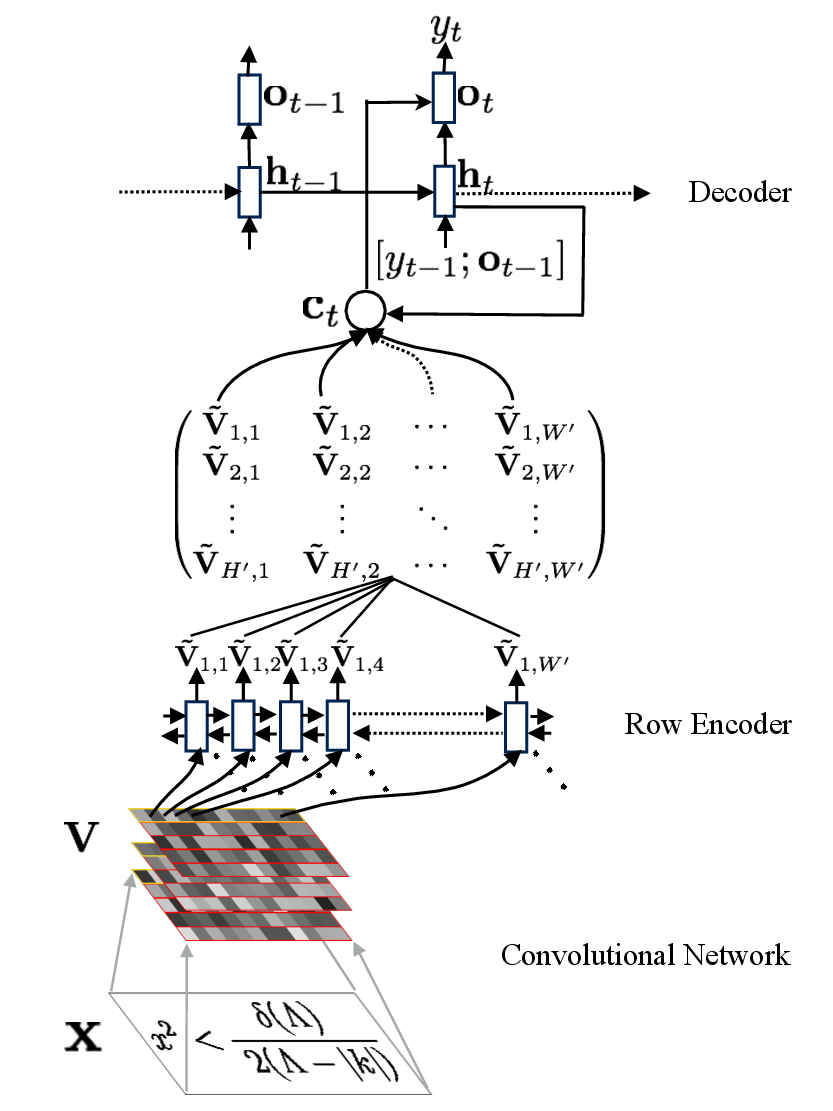
\includegraphics[width=0.5\textwidth]{neural-network.png}
  \caption{Neural network used by \cite{1609.04938} to decompile \LaTeX{}.}
\end{figure}

Their model begins with a 6 layer CNN. As alluded to earlier, CNN's have a great
ability to extract information from images. This is exemplified by Yan LeCun
\textit{et al.} in\cite{lecun_bottou_bengio_haffner_1998} where they used it
to achieve cutting edge performance in optical character recognition. Again,
it shines in classifying images in \cite{NIPS2012_4824} and \cite{szegedy2013deep}.
It is also used in video tagging \cite{karpathy2014large}.

Although CNN's are good at classifying, it is not very good at extracting semantics
from data. This is why the RNN is used. By tokenizing the \LaTeX{} alphabet, it
is possible to used the output of the CNN to drive a ``translation'' machine.
Translation in the sense that it is taking pictures and outputting a new format
with the same semantic meaning. RNN's are used heavily in translation tasks.
In \cite{1406.1078}, Cho \textit{et al.} introduced a new scheme called
sequence-to-sequence (seq2seq) that allows for arbitrary length of inputs and outputs.
This is a desirable trait for our network to have as mathematical equations have
unspecified lengths. Finally, the last thing that \cite{1609.04938} uses in their
\LaTeX{} decompiler is an attention-based encoder-decoder which was introduced by
Bahdanau, Cho, and Bengio in \cite{1409.0473}. This encoder-decoder allows
the output to be a weighted combination of all of the inputs, not just the immediately
preceding one. Again, this is useful in mathematical equations as the output could
be a function of many neighbouring inputs. An example of this is the integral. Once
an integral sign appears, the likelihood of $dx$ appearing is very high. However,
it appears much after the integral sign, thus, an attention-based mechanism allows
for the neural network to keep emphasis on the integral sign until the $dx$ has appeared.

\section*{Problem}

The problem at hand is given a black and white image, $x \in \mathcal{X}$, of written formulae
and a \LaTeX{} source $y \in \mathcal{Y}$, we wish to find a function $f$ such that
the 1/0 risk is minimized. In notation,
$$
  \arg\min_{f \in \mathcal{F}} \sum_{i=1}^n 1_{y_i \neq f(x_i)}
$$
More specifically, the functional class $\mathcal{F}$ is the neural network we
create and all of its potential weights, $\mathcal{X}$ are images with a certain
width and height, and $\mathcal{Y}$ are sequences of tokens that comprise a \LaTeX{}
equation.

\section*{Model}

As said previously, the model we used was greatly influenced by \cite{1609.04938} and we define
the precise network we used. The first step is to create a batch of images. We used a batch size of
2 as we did not have a lot of data. We also batched the images so that they had similar
sizes to the other images in the optimization step to aid with training. Next, it was passed
through 6 convolutional layers and 4 pooling layers. Table 1 shows the exact parameterization
of the layers. Finally, we used ReLU for the activation units.

\begin{table}[t]
  \caption{CNN layers description. c: number of filters, k: kernel size, s: stride, p: padding, po: pooling size, bn: batch normalization.}
  \centering
  \begin{tabular}{c c}
    \toprule
    \textbf{Conv} & \textbf{Pool}               \\
    \cmidrule{1-2}
    c:512, k:(3,3), s(1,1), p(0,0), bn & - \\
    c:512, k:(3,3), s(1,1), p(1,1), bn & po:(1,2), s:(1,2), p:(0,0) \\
    c:256, k:(3,3), s(1,1), p(1,1) & po:(2,1), s:(2,1), p:(0,0) \\
    c:256, k:(3,3), s(1,1), p(1,1), bn & - \\
    c:128, k:(3,3), s(1,1), p(1,1) & po:(2,2), s:(2,2), p:(0,0) \\
    c:64, k:(3,3), s(1,1), p(1,1) & po:(2,2), s:(2,2), p:(2,2) \\
    \bottomrule
  \end{tabular}
\end{table}

After the CNN, they are fed into the row encoder. As mentioned before, the row encoder follows
an attention-based mechanism. In this specific implementation, the rows of the CNN layer are
fed into the encoder. The reasoning being that equations are read mostly laterally. This is repeated for every
row of the CNN output and the encoder produces an equally sized output. To achieve the
attention, the encoder is fed into the decoder in such a way that the decoder can
influence which parts of the encoder are important. Essentially, it is a backward
feedback mechanism that allows the hidden state of the decoder to specify which
neighbouring features are the most important.

Finally, we get to the decoder. The decoder has an initial input. It is a
special token called \texttt{START}. This is coupled with the output of the encoder to produce
the next predicted token. This new token is then used as input to the decoder. This is iteratively
applied until the decoder produces another special token called \texttt{END}. At this point,
the prediction process is done. Again, to be able to batch unequally sized formulas, we introduced
a third special token called \texttt{PADDING}. This works similarly to \texttt{END} in
the sense that the prediction process should stop when the decoder outputs \texttt{PADDING}.
Implementation wise, we again followed the exact model in \cite{1609.04938} and used
a bidirection RNN for the encoder with a hidden state of size 256. The decoder was
of size 512 with token embeddings of size 80. Finally, the individual cells of the RNN's
were comprised of Long-Short Term Memory cells.

\section*{Data}

We used a the \texttt{IM2LATEX-100K} dataset that provides 103,556 different
\LaTeX{} equations coupled with their compiled pdf images. However, no dataset
exists for handwritten equations. Thus, we set out to use the \texttt{IM2LATEX-100K}
as the labels for our new dataset and to generate the inputs. To speed up the process
of collecting the data, we created an iPad app that displayed equations from the
\texttt{IM2LATEX-100K}. We could then input the equation via the iPad and then
download the images at the press of a button. Figure 2 shows the layout of the app.
The top half displays the equation, the bottom half for writing (empty in this screenshot),
and a couple of buttons for minor editing capabilities. While much faster than alternative
methods, only 500 equations were collected.

\begin{figure}[h]
  \centering
  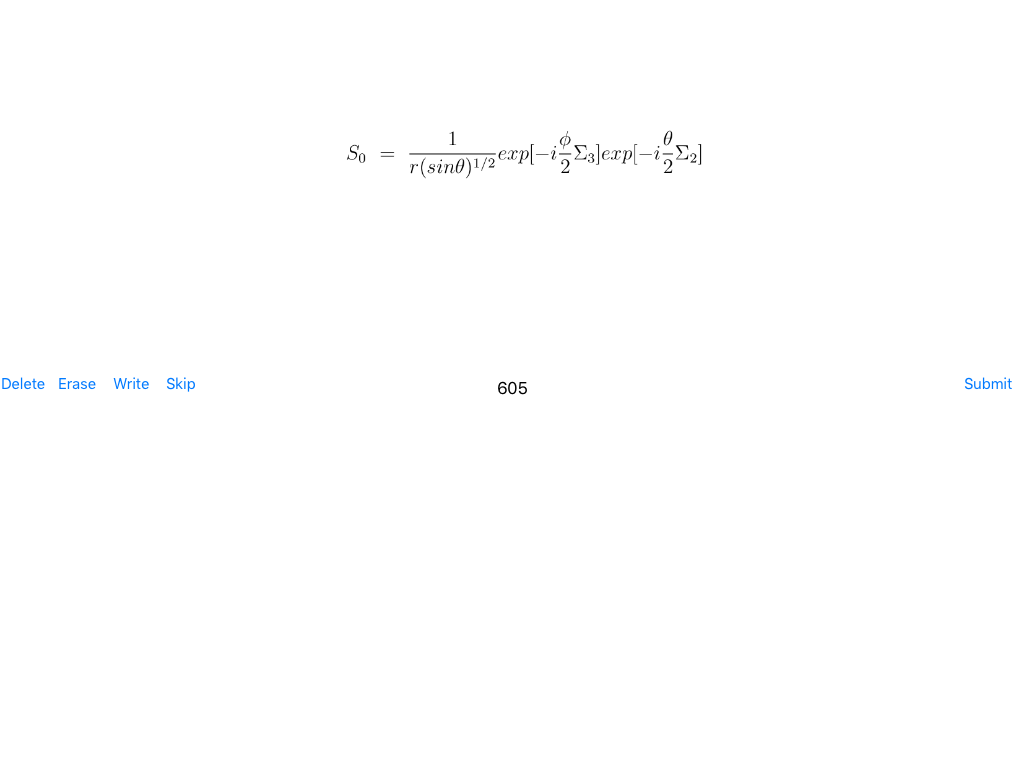
\includegraphics[width=0.6\textwidth]{ipad-app.png}
  \caption{Screen shot of the app created to gather data.}
\end{figure}

After the data was collected, preprocessing needed to be done. The main issue
that needs to be dealt with is to reduce the size of images. Thus, the first thing
we did was to find the smallest bounding box and add a 8 pixel padding so that the
CNN doesn't suffer from features being located on the edges. Figure 3 shows an example
of a preprocessed input.

\begin{figure}[h]
  \centering
  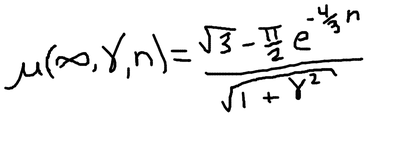
\includegraphics[width=0.6\textwidth]{example-input.png}
  \caption{Preprocessed input image.}
\end{figure}

Another issue is that images should be batches together relative to the similar sizes to
reduce the amount of padding that needs to be done. Thus, a custom batching step was created
to sort the images according to size and batch the images most similar in size. On the equation
side, there are many different normalization techniques that can be used. We opted
to follow the steps in \cite{1609.04938} and normalize all the equations. For example,
ensuring that subscript is before superscript is one such correction. Finally, we
opted to use a word based tokenization of \LaTeX{} equations as opposed to individual
characters. That is, `\\sigma' is considered to be one token even though it takes
6 characters. This was justified because the \LaTeX{} symbols are what is rendered
into the image. Finally, we went over the \texttt{IM2LATEX-100K} dataset and collected
all the symbols and tokenized them. We then removed any token that was used only once.

\section*{Training}

Training was done on an Amazon AWS EC2 instance with a NVIDIA Tesla K80 to achieve
maximum performance. Even with this GPU, training takes a day and is most likely due to
the fact of the small dataset. Implementation wise, 80\% of the data was used as training
samples and 10\% of the data was used for validation. After each batched gradient descent, we used the Adadelta method, the
validation set was used to assess the current neural net. If it's accuracy increased,
the current step sized was not changed, if it did not increase twice in a row, the step size
was reduced. The last 10\% of the data was used for testing. The algorithm was not trained on this
data at any point in the optimization process. We only use this last 10\% to quantify
any claims.

\section*{Results}

After almost a full day of training, we get that the word accuracy of our model is
25\%. This is below the 75\% accuracy that the model we based ours on got on the
\texttt{IM2LATEX-100K} or the 95\% achieved by cutting edge OCR techniques. While
this is not the result we wanted, we speculate that the entire gap from 25\% to
75\% would be reconciled if we had a proper dataset with tens of thousands of data points.
Despite the lack of performance, the loss function did systematically get smaller as seen
in Figure 4.

One interesting thing to note of the predictions is that they all seem to learn
that if one has a padded equation, then the padding always goes at the end. There
is never a padding that occurs in the middle. Furthermore, the predictions also know
that an equal sign goes somewhere in the middle of the equation and often puts a couple
of equal signs in the middle to hedge its bets on where exactly it is. That is, you see
many predictions of the form

$$
  \texttt{START} \rightarrow ... \rightarrow = \rightarrow = \rightarrow = \rightarrow ... \rightarrow \texttt{END}
$$

\begin{figure}[h]
  \centering
  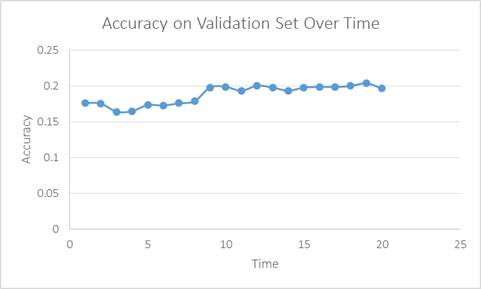
\includegraphics[width=0.6\textwidth]{accuracy.png}
  \caption{Accuracy over time.}
\end{figure}

\section*{Conclusion}

While this method did not achieve state of the art performance, it does provide
some positives. For one, it shows the versatility of the model we used. The model
is able to generalize the problem of going from images to some type of syntactic
language. Secondly, as the loss kept diminishing throughout the entire training
period, it hints that more time would have allows the neural net to converge to
something better than the result achieved. However, ultimately, better results
and a larger dataset go hand in hand. Finally, based on the results of the predictions,
using 0/1 loss may have been counterproductive of the goal and resulted in the behaviour
seen. That is, with 0/1 loss, the hard assignment forces the neural net to try
and get the most number of tokens correct as opposed to confusing the token with
a similar looking token, say $x$ and $X$. Thus, it encourages the neural net
to weight the most common symbols such as $=$, $\{$, and $\}$ more heavily. It would
be a great extension of this project to see the effects of different loss functions
on the prediction outcomes.

\section*{References}

\small

\bibliographystyle{ieeetr}
\begingroup\renewcommand{\section}[2]{}
\bibliography{references.bib}
\endgroup

\end{document}
